%!TEX root = ../main.tex

\chapter{Finding unreachable code using a SMT-Solver \textasciitilde 10 sites}
\label{cha:finding unreachable code using a smt-solver}
\emph{10 Sites}

The developed approach uses the \emph{Control-flow graph} as a basis like described in \ref{sec:building cfg}, but does not transform it into \emph{Single static Assignment} form.
During analysis the \emph{Control-flow graph} will be traversed and interpreted like the program will be executed.
After each interpretation state (e.g. \emph{Assignments}, \emph{Path Conditions}) will be added accordingly and must be taken into account.
Merging of state has to be handled correctly to make correct statements about the current value of a variable.
The state is represented in the form of a predicate, which may be checked by a system capable of determining satisfiability (e.g. an \emph{SMT-Solver}).
Satisfiable results will continue with the next block(s) and using the new state as a basis and flag this block as visitable.
Unsatisfiable results stop the computation at the current block and will not pursue to continue the path.
Therefore this method is pessimistic.
By using this method every error should be found in theory (as described in \ref{cha:conclusion}), since every instruction will be handled like during execution. 
This entails barriers such as: 
\begin{itemize}
	\item Significant increase in time needed for analysis. 
	\item Possibly exponentially growing expressions to determine satisfiability.
\end{itemize}
These problems lead to greater execution time, which requires the implementation of reactions (e.g. early stopping, assuming values for variables in loops).

% \section{Analysis}
% \subsection{Foundation \textasciitilde 1 site}
% \subsection{State-management \textasciitilde 3 site}
% \subsection{Creating combined SMT-Lib-Statements \textasciitilde 1 site}
% \subsection{Interpret Result of SMT-Solver \textasciitilde 1 site}


\section{Translation of Functions}
\label{sec:translation}
For every function the \emph{Control-flow Graph} will be calculated and used as basis. Information about parameters and global-/system variables also need to be provided in order to handle Function-/Procedure-calls. 
Two separate procedures will be performed on this Control-flow Graph.
\begin{enumerate}
	\item \emph{Unreachable Code due to unconditional jumps} is relatively easy to find after the Control-flow Graph was created. Every Block (except the \emph{Begin Block}) which does not have any incoming edges must be unreachable.
		Note that these types of errors may also be found as described in section \ref{sec:analysis}, but were filtered out before.
	\item \emph{Unreachable Code due to infeasible conditions} needs a sophisticated and more expensive (in terms of computing resources) approach to identify. The following section \ref{sec:analysis} describes how to detect them.
\end{enumerate}
\subsection{Translation of Instructions}
% Types of instructions
Instructions come in three different types and must be marked accordingly:
\begin{enumerate}
	\item \emph{Assignments} are usually the most common form of instruction. They denote a change of the underlying value of a variable and therefore reset the state (of said variable) during analysis. 
	\item \emph{Conditions} occur only as the last instruction of a block from a \emph{Control-flow Graph}. Note that the last Instruction does not necessarily to be a \emph{condition}.
	\item \emph{Procedure Calls} may be mutable and could change variables, if they a are applied as \emph{Output-Parameters}. Procedure Calls will be dissolved into \emph{Assignments} during analysis.
\end{enumerate}
% AST-Object representation of instructions
Every Instruction will also be represented in an \emph{Abstract-Syntax-Tree}-like notation. Each Symbol, for example a variable, name of a function or any given literal (like numbers and strings), are represented as an \emph{BaseObject}. Functions are, in fact, just a special form of this \emph{BaseObject}, which may contain variables. Functions are not only direct function-/procedure Calls, but also operations (like \emph{+} and \emph{-}). User-defined Functions will also be represented as a special form of the described \emph{FunctionObject} before, which contain the declaration of parameters (since Named Parameters are a language feature of IEC and therefore must be handled correctly), which will be - again - represented as \emph{BaseObjects}. 
 


\begin{figure}[h!]
	\centering
	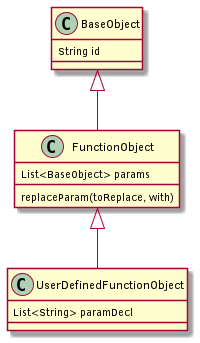
\includegraphics[width=0.2\textwidth]{SMTObject}
	\caption{\emph{AST}-like representation of instructions. This kind of representation makes it easy to work with, since it is a very easy, tree-like data-structure which may be traversed easily. Not only replacing variables and values may be done effortlessly, but also the generation of \emph{SMT-Lib} Code, since this representation is similar to \emph{LISP}.}
	\label{fig:smtobject}
\end{figure}
\section{Analysis}
\label{sec:analysis}


\subsection{Interpretation of Instructions}
% Handling of Ass, Cond, Proc and state management
% Creation of SMT-Statements
% Early Stopping
% 